\section{Perintah Navigasi}
Sebelum melakukan perintah navigasi pastikan kita memiliki tools Spyder, anaconda dan selenium. Lakukan instalasi selenium dengan cara ketik "pip install selenium" pada anaconda.

kemudian buka aplikasi Spyder dan masukkan program berikut ini :
\begin{verbatim}
from selenium import webdriver
opsi = webdriver.firefox.options.Options()
opsi.headless = False
binary = webdriver.firefox.firefox_binary.FirefoxBinary('C:\\Program Files\\Mozilla Firefox\\firefox.exe')
cap = webdriver.common.desired_capabilities.DesiredCapabilities().FIREFOX
cap['marionette'] = True
browser=webdriver.Firefox(options=opsi,capabilities=cap,firefox_binary=binary)
browser.get('https://tokoperhutani.com/')
\end{verbatim}

Penjelasan : 
\begin{enumerate}
    \item From selenium import webdriver Modul selenium webdriver mengimplementasikan kelas yang mendukung berbagai browser termasuk Firefox, Chrome, Internet Explorer, Safari, yang lain, dan RemoteWebDri	ver juga untuk menguji pada browser yang tersedia di mesin jarak jauh. Kita perlu mengimpor webdriver dari paket Selenium untuk menggunakan metode Selenium WebDriver.
    \item Opsi adalah kelas dalam paket webdriver selenium firefox. opts adalah turunan dari kelas Opsi yang dipakai untuk program.
    \item Headless, Python memperbarui instance Options, untuk menyimpan informasi "pengguna ini ingin memulai instance browser headless”.
    \item Webdriver.common.desiredcapabilities.DesiredCapabilities().FIREFOX.   sebagai titik awal untuk membuat objek kemampuan yang diinginkan untuk meminta driver web jarak jauh untuk terhubung ke server selenium.  
    \item Marionette adalah driver otomatisasi untuk mesin Gecko Mozilla.
    \item Browser.get metode akan menavigasi ke halaman yang diberikan oleh URL. WebDriver akan menunggu hingga halaman dimuat penuh (yaitu, "onload" telah diaktifkan) sebelum mengembalikan kontrol ke tes atau skrip.
\end{enumerate}

Setelah anda membuat Tambahan Codingan  seperti diatas untuk merunning program anda tekan run pada bar diatas. Saat kotak yang ditandai pada gambar dibawah, berwarna merah artinya proses running program tersebut masih berjalan. Setelah program di run akan otomatis membuka Mozila Firefox dan akan langsung membuka website tokoperhutani secara otomatis.

\begin{figure}[h]
\centering
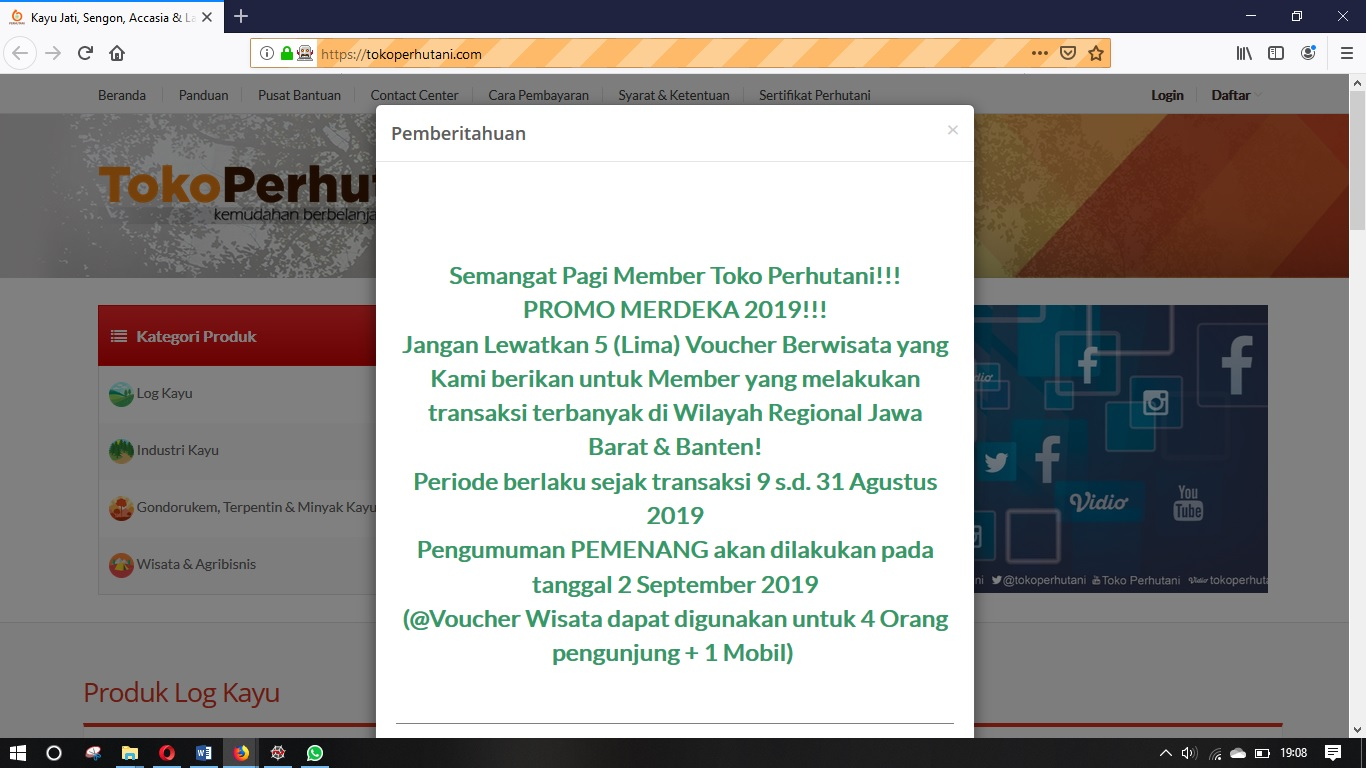
\includegraphics[scale=0.3]{figures/1x}
\caption{Navigator Pada Menu Beranda}
\end{figure}

Masukkan code berikut untuk test navigator pada menu Cara Pembayaran :

\begin{verbatim}
  carapembayaran= browser.get('https://tokoperhutani.com/article/static_art/cara-pembayaran'
\end{verbatim}

Hasilnya  di Mozilla Akan mucul seperti ini :
\begin{figure}[h]
\centering
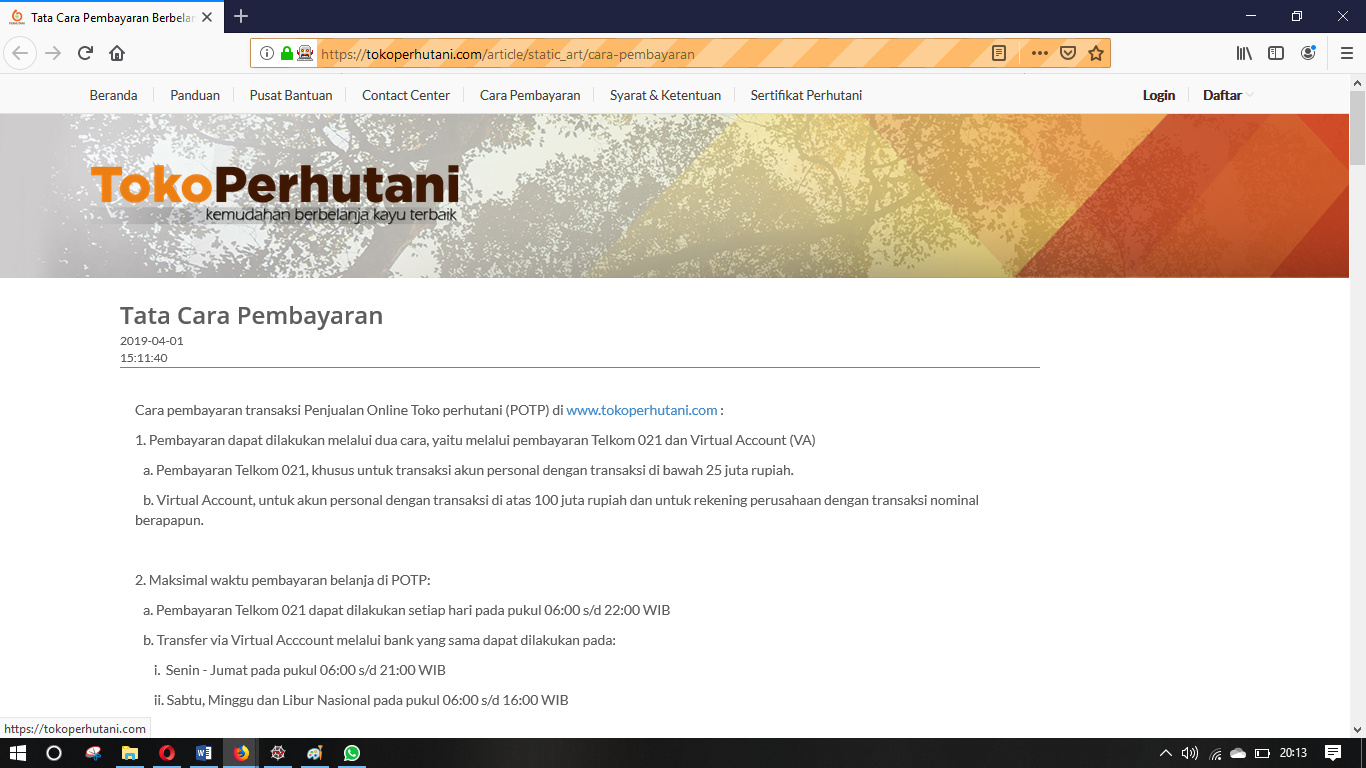
\includegraphics[scale=0.3]{figures/2}
\caption{Tata Cara Pembayaran}
\end{figure}

Masukkan code berikut untuk test navigator pada menu Sertifikat Perhutani :

\begin{verbatim}
  sertifikatperhutani= browser.get('https://tokoperhutani.com/SertifikatPerhutani')
\end{verbatim}

Hasilnya  di Mozilla Akan mucul seperti ini :
\begin{figure}[h]
\centering
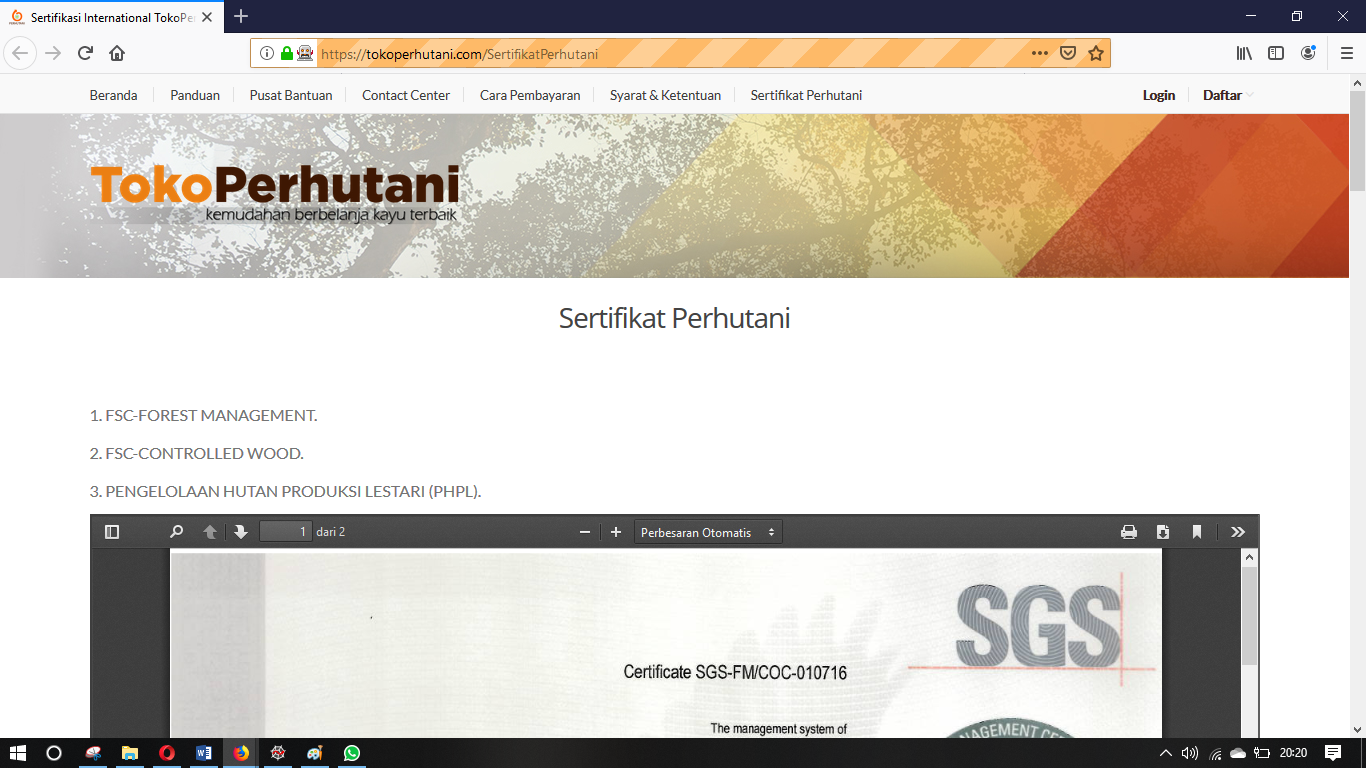
\includegraphics[scale=0.3]{figures/3}
\caption{Navigator Pada Sertifikat Perhutani}
\end{figure}

Masukkan code berikut untuk test navigator pada menu  Panduan:
\begin{verbatim}
  panduan = browser.get('https://tokoperhutani.com/panduan')
\end{verbatim}

Hasilnya  di Mozilla Akan mucul seperti ini :
\begin{figure}[h]
\centering
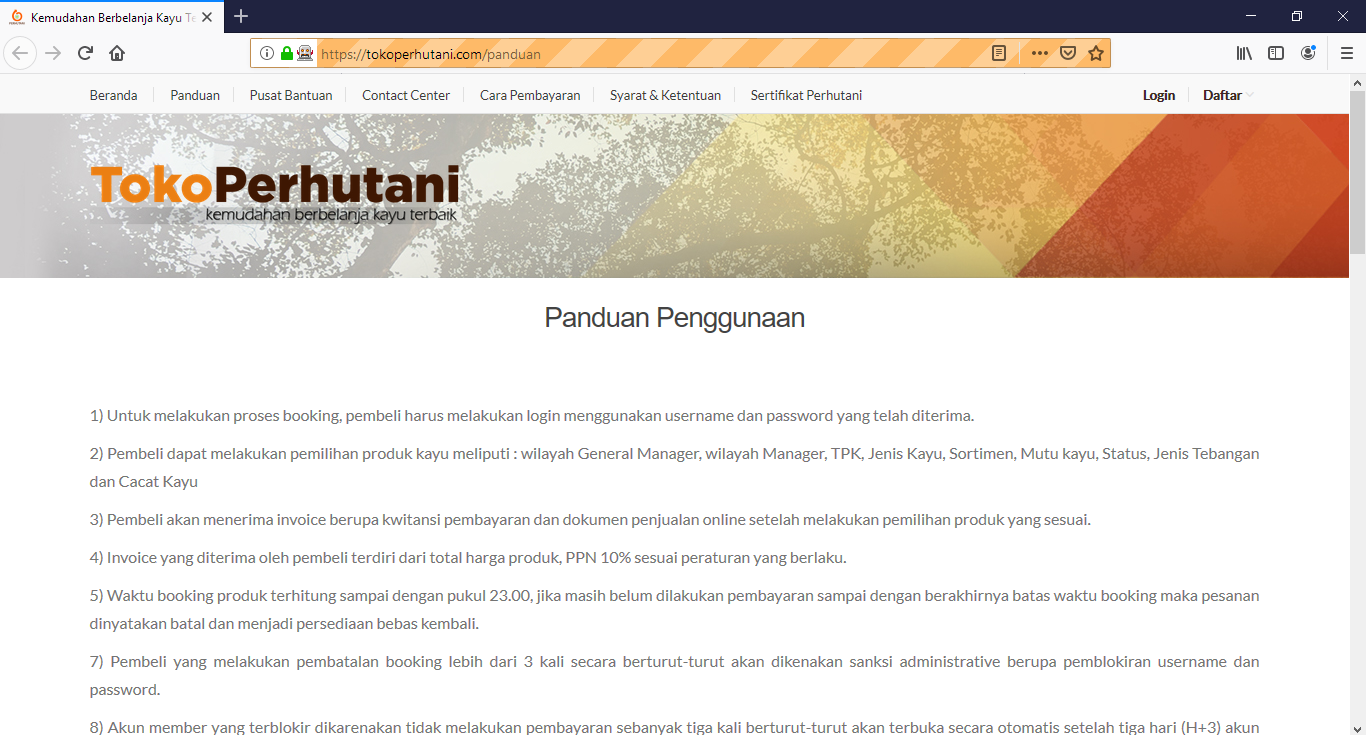
\includegraphics[scale=0.3]{figures/1hasil.PNG}
\caption{Navigator Pada Panduan}
\end{figure}

Masukkan code berikut untuk test navigator pada menu  Pusat bantuan:
\begin{verbatim}
  pusatbantuan = browser.get('https://tokoperhutani.com/faqs')
\end{verbatim}

Hasilnya  di Mozilla Akan mucul seperti ini :
\begin{figure}[h]
\centering
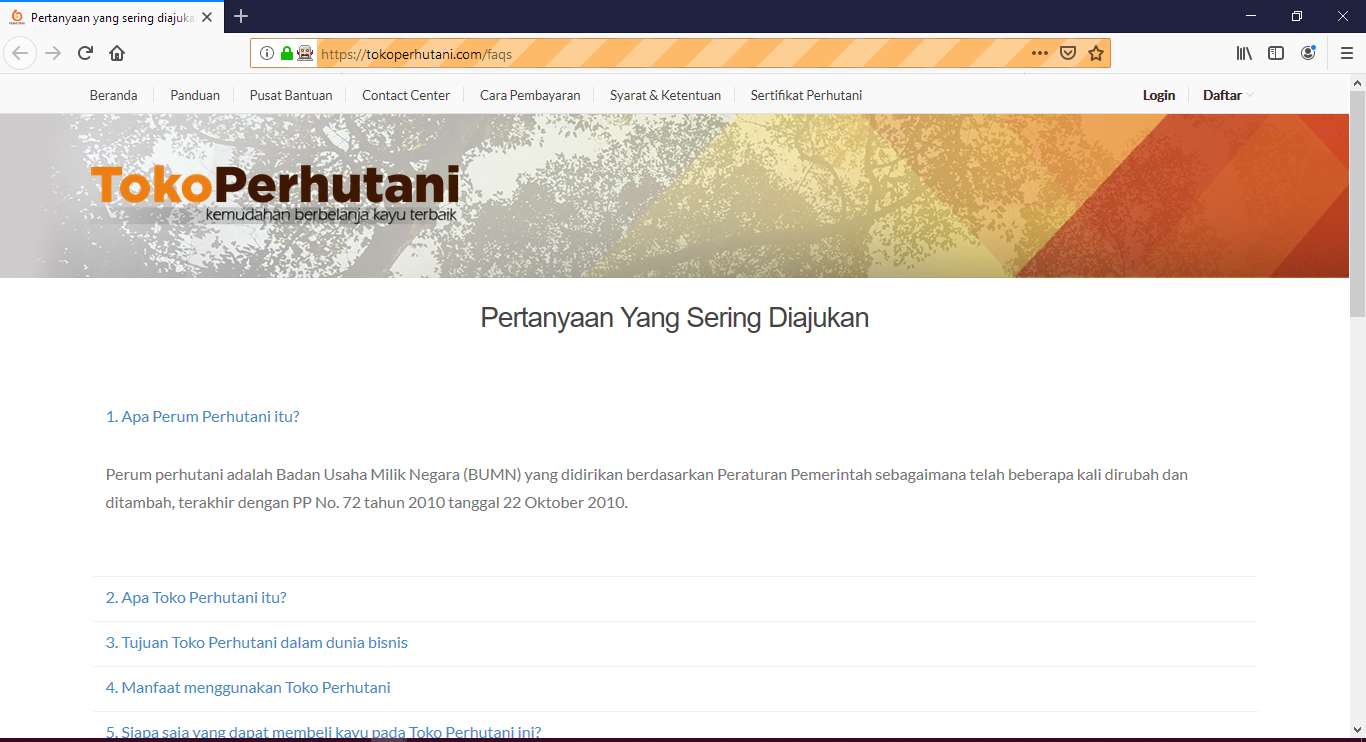
\includegraphics[scale=0.3]{figures/2hasil.PNG}
\caption{Navigator Pada Pusat Bantuan}
\end{figure}

Masukkan code berikut untuk test navigator pada menu  Alamat kantor:
\begin{verbatim}
  alamatkantor = browser.get('https://tokoperhutani.com/article/detil/alamat-kantor')
\end{verbatim}

Hasilnya  di Mozilla Akan mucul seperti ini :
\begin{figure}[h]
\centering
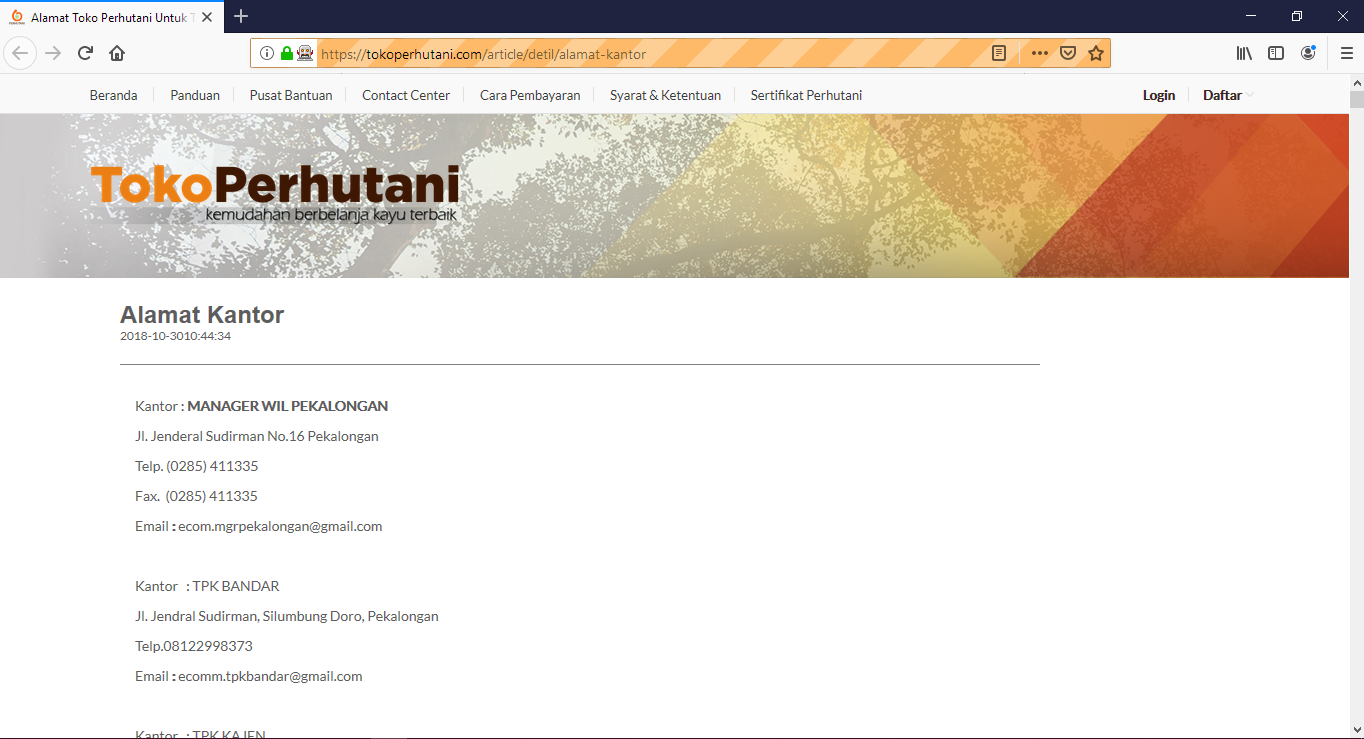
\includegraphics[scale=0.3]{figures/3hasil.PNG}
\caption{Navigator Pada Alamat Kantor}
\end{figure}
\\

Masukkan code berikut untuk test navigator ke halaman panduan Registrasi:
\begin{verbatim}
  browser.find_element_by_link_text('Registrasi').click()
\end{verbatim}

Hasilnya  di Google Chrome Akan mucul seperti ini :
\begin{figure}[h]
\centering
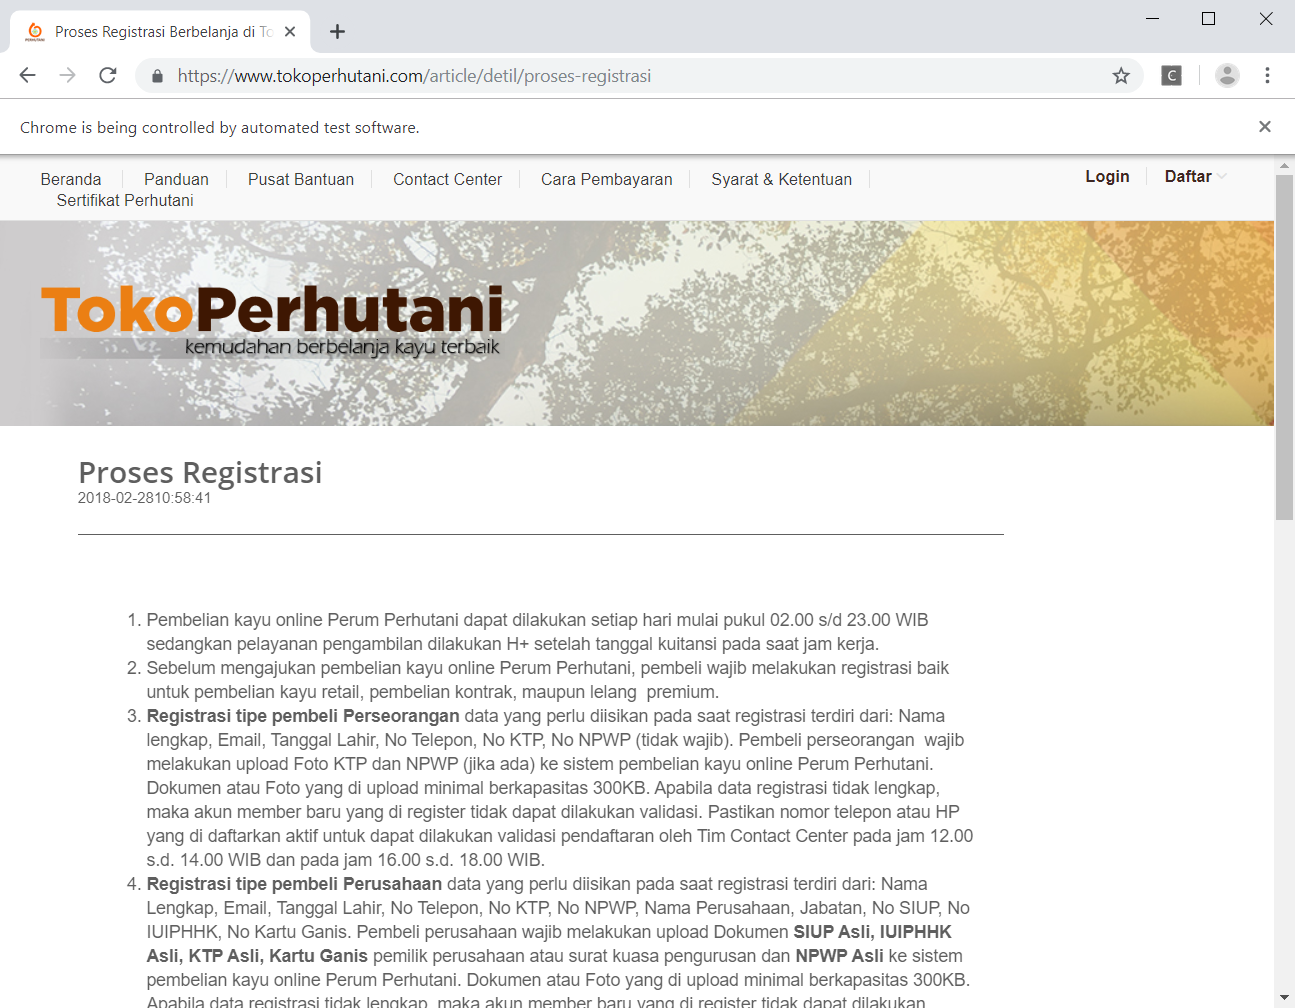
\includegraphics[scale=0.3]{figures/1pdregis}
\caption{Halaman Panduan Registrasi}
\end{figure}

Masukkan code berikut untuk test menampilkan pilihan pendaftaran:
\begin{verbatim}
  browser.find_element_by_link_text('Daftar').click()
\end{verbatim}

Hasilnya  di Google Chrome Akan mucul seperti ini :
\begin{figure}[h]
\centering
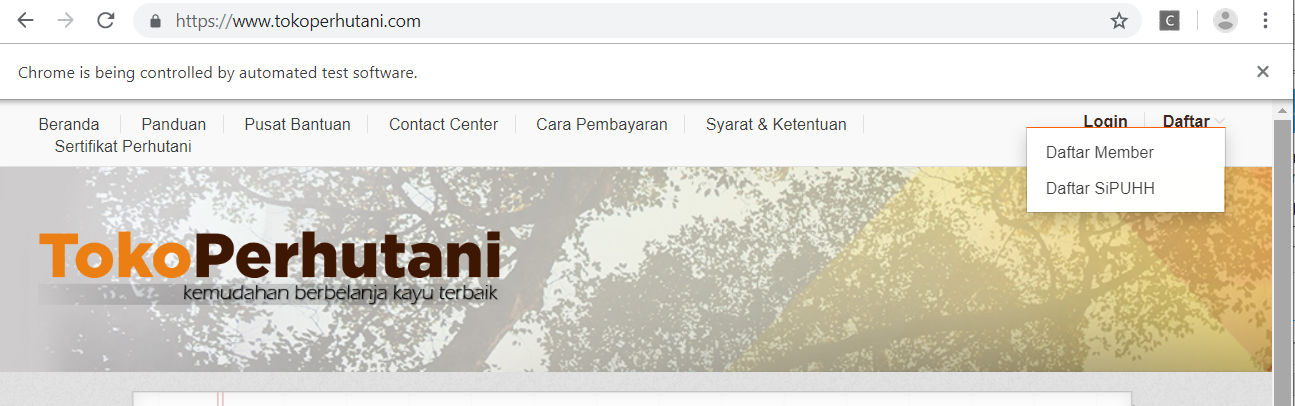
\includegraphics[scale=0.3]{figures/2daftar}
\caption{Tombol navigasi Daftar}
\end{figure}

Masukkan code berikut untuk test memilih Daftar member:
\begin{verbatim}
  browser.find_element_by_link_text('Daftar Member').click()
\end{verbatim}

Hasilnya  di Google Chrome Akan mucul seperti ini :
\begin{figure}[h]
\centering
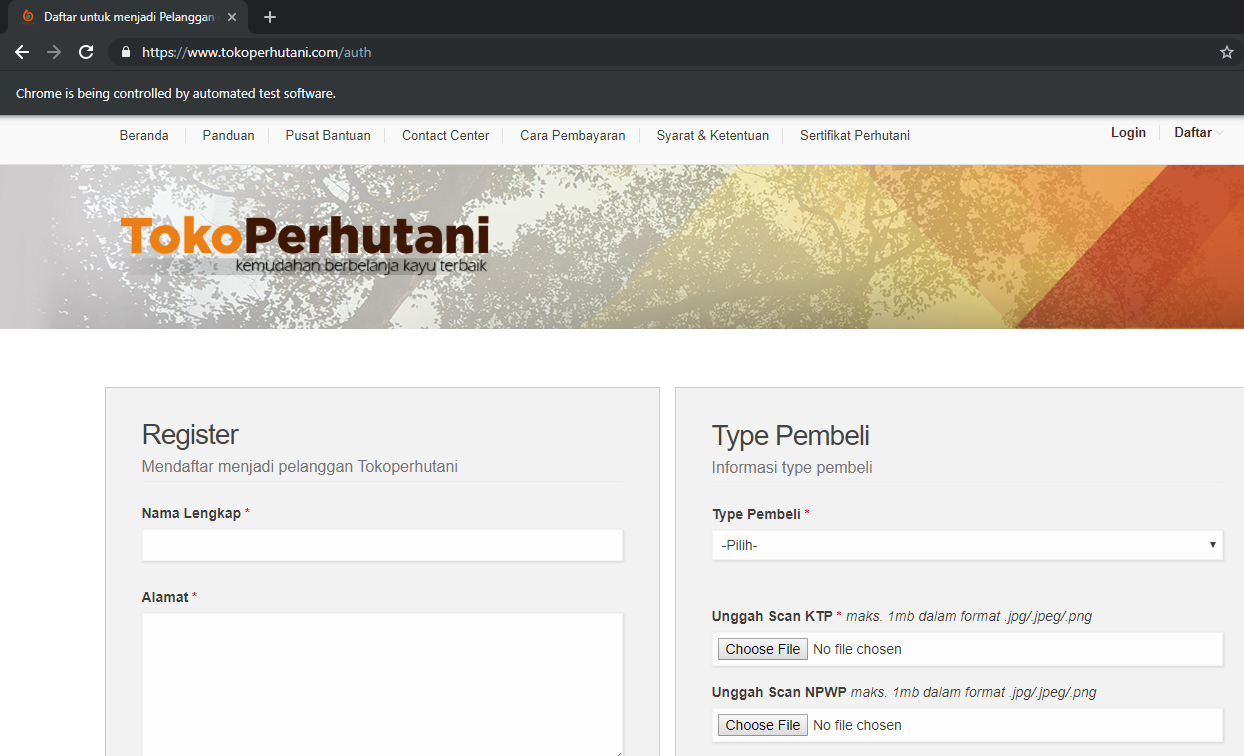
\includegraphics[scale=0.3]{figures/3daftar}
\caption{Halaman Daftar Member}
\end{figure}

Masukkan code berikut untuk test navigator ke halaman Contact Center:
\begin{verbatim}
  browser.find_element_by_link_text('Contact Center').click()
\end{verbatim}

Hasilnya  di Google Chrome Akan mucul seperti ini :
\begin{figure}[h]
	\centering
	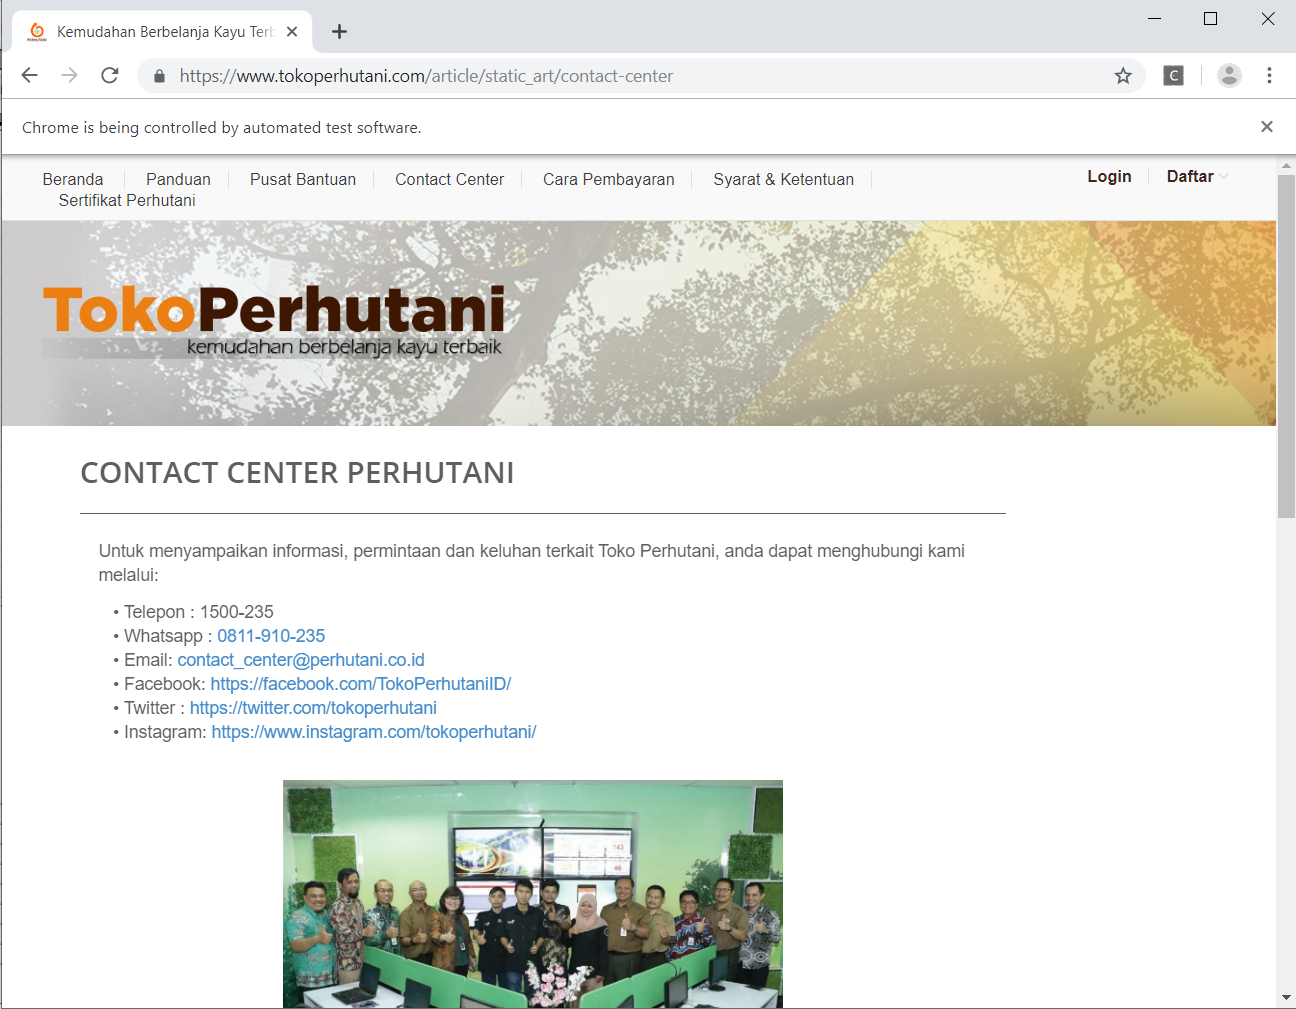
\includegraphics[scale=0.3]{figures/4kontak}
	\caption{Halaman Contact Center}
\end{figure}

Masukkan code berikut untuk test navigator pada menu Kayu Pinus:

\begin{verbatim}
  KayuPinus = browser.get('https://tokoperhutani.com/article/detil/kayu-pinus'
\end{verbatim}

Hasilnya  di Mozilla Akan mucul seperti ini :
\begin{figure}[h]
\centering
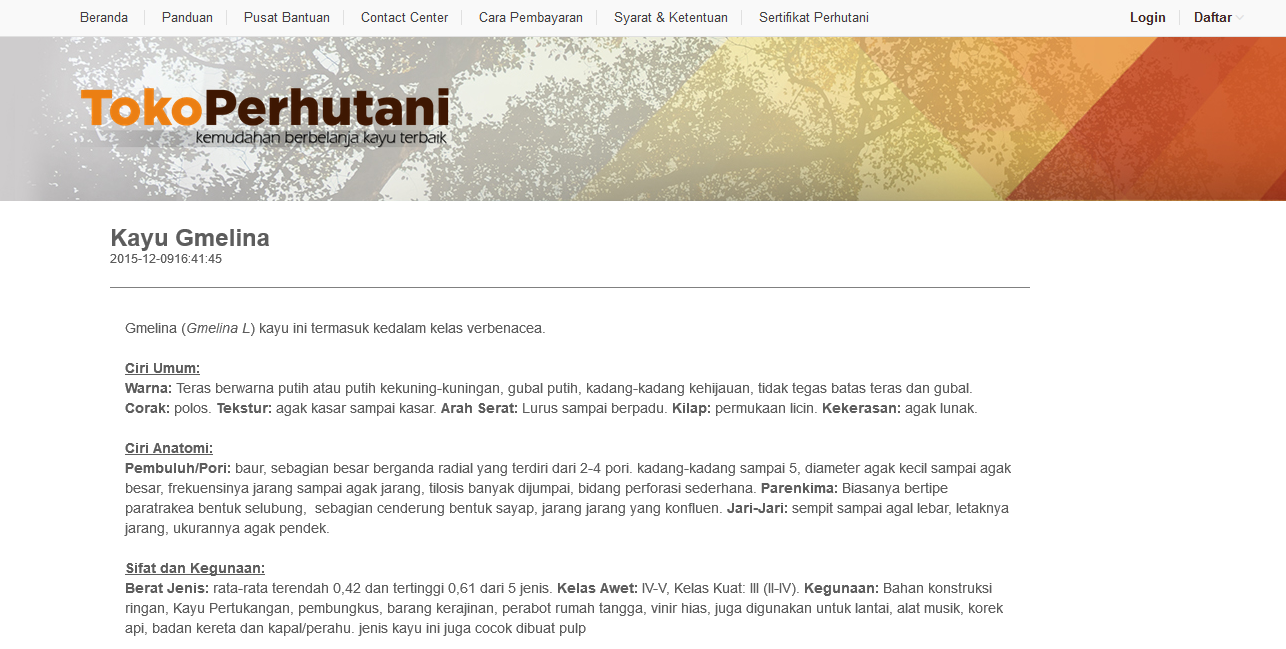
\includegraphics[scale=0.3]{figures/aa}
\caption{Kayu Pinus}
\end{figure}

Masukkan code berikut untuk test navigator pada menu Kayu Gamelina :
\begin{verbatim}
  KayuGmelina = browser.get('https://tokoperhutani.com/article/detil/kayu-gmelina'
\end{verbatim}

Hasilnya  di Mozilla Akan mucul seperti ini :
\begin{figure}[h]
\centering
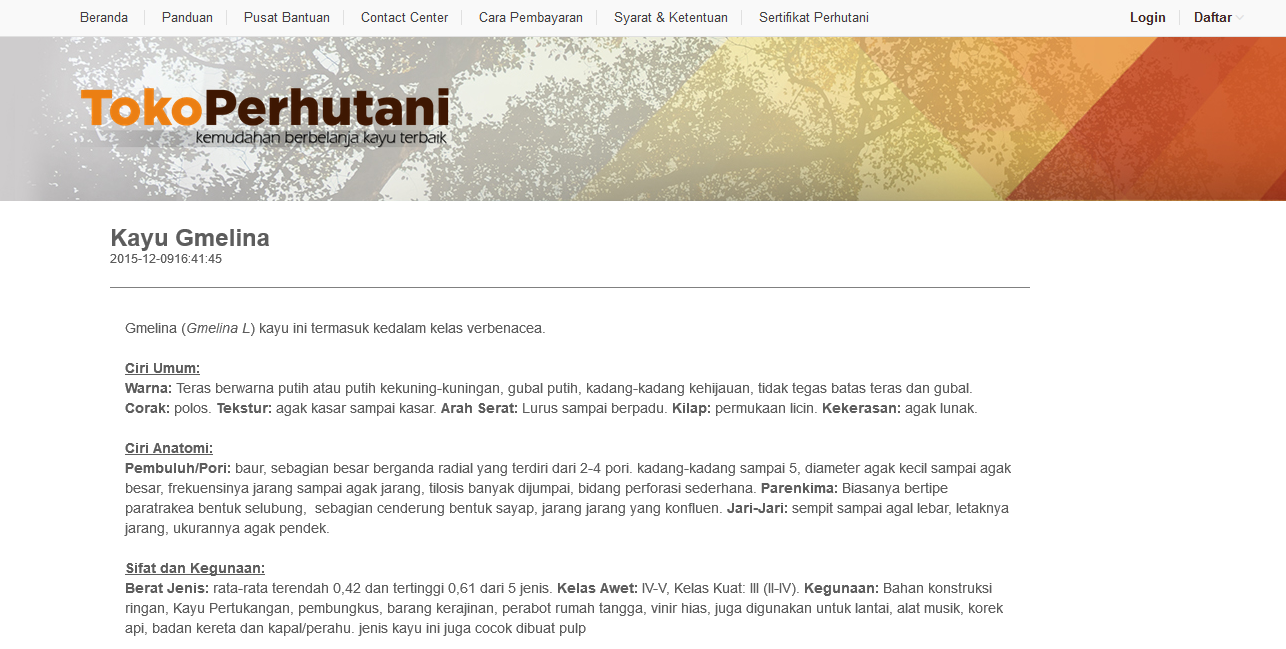
\includegraphics[scale=0.3]{figures/2kg}
\caption{Kayu Gamelina}
\end{figure}

Masukkan code berikut untuk test navigator pada menu Kayu Sonokeling :
\begin{verbatim}
  KayuSonokeling = browser.get('https://tokoperhutani.com/article/detil/kayu-sonokeling'
\end{verbatim}

Hasilnya  di Mozilla Akan mucul seperti ini :
\begin{figure}[h]
\centering
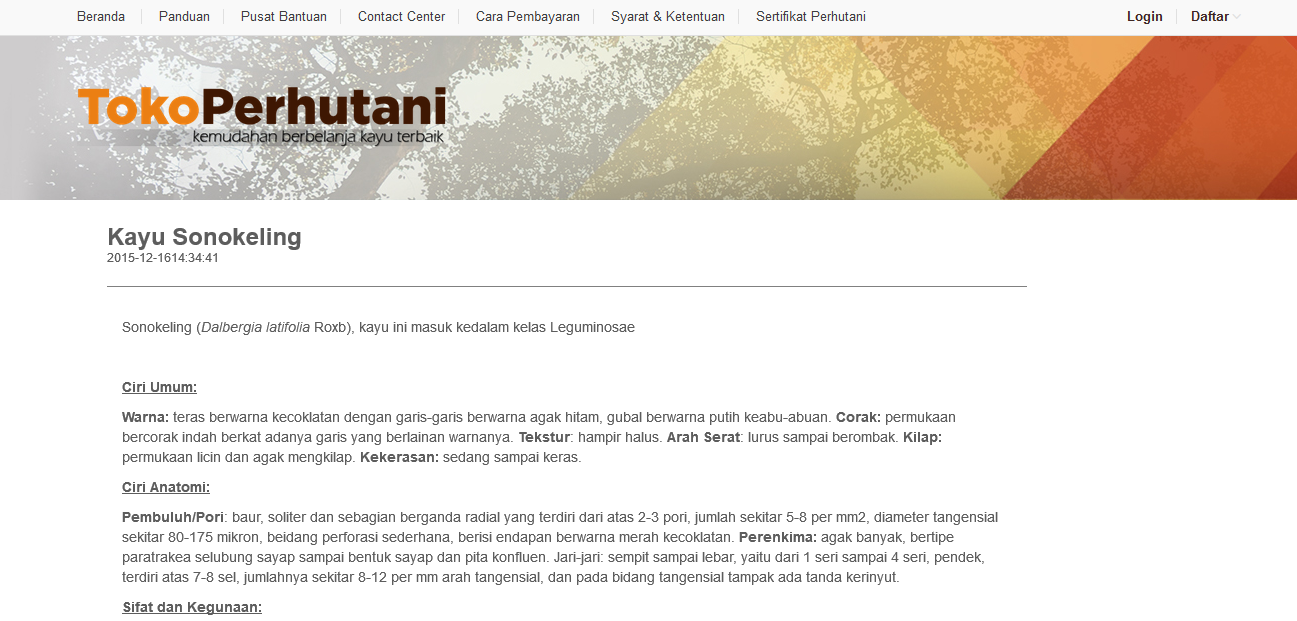
\includegraphics[scale=0.3]{figures/cc}
\caption{Kayu Sonokeling}
\end{figure}

Masukkan code berikut untuk test navigator pada menu Kayu Pinus :
\begin{verbatim}
  kayupinus = browser.get('https://www.tokoperhutani.com/article/detil/kayu-pinus')
\end{verbatim}

Hasilnya  di Mozilla Akan mucul seperti ini :
\begin{figure}[h]
\centering
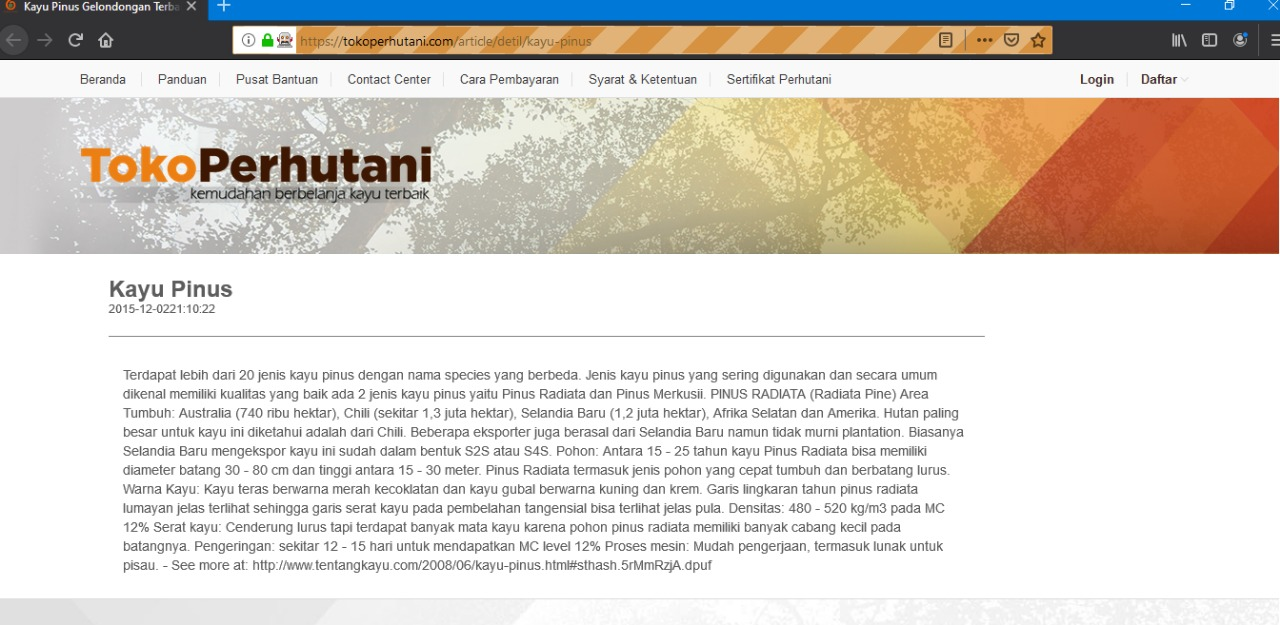
\includegraphics[scale=0.3]{figures/j1}
\caption{Kayu Pinus}
\end{figure}

Masukkan code berikut untuk test navigator pada menu Kayu Gmelina :
\begin{verbatim}
  kayugmelina  = browser.get('https://www.tokoperhutani.com/article/detil/kayu-gmelina')
\end{verbatim}

Hasilnya  di Mozilla Akan mucul seperti ini :
\begin{figure}[h]
\centering
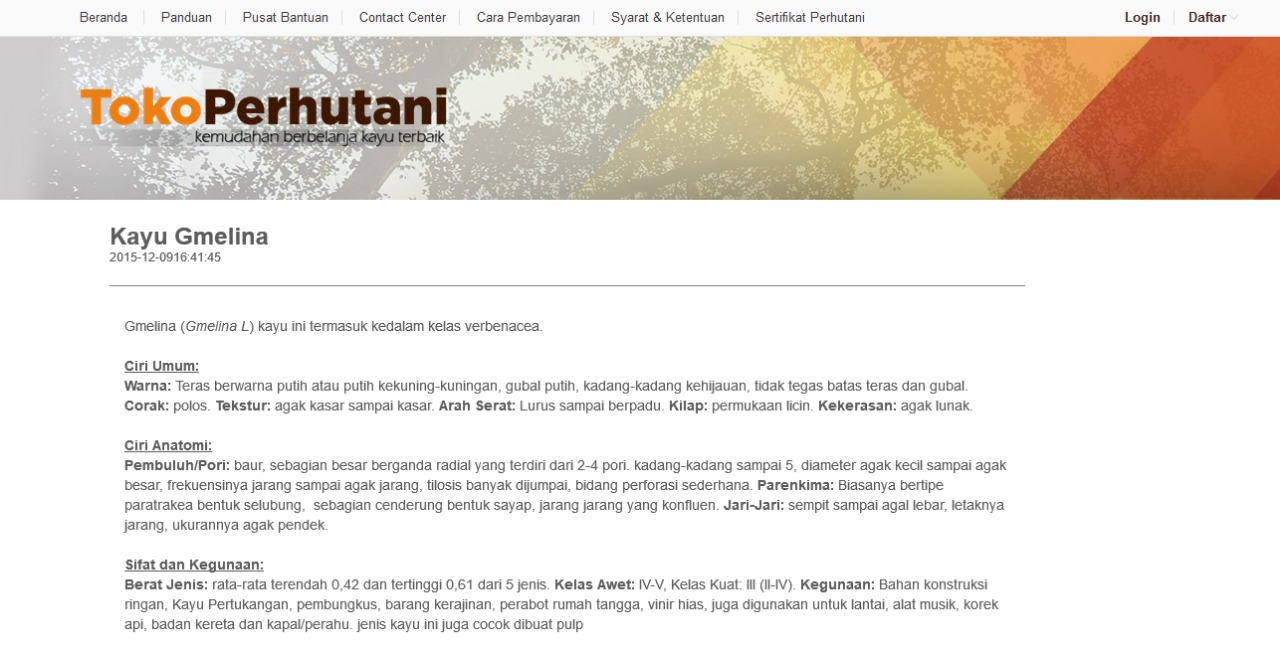
\includegraphics[scale=0.3]{figures/j2}
\caption{Kayu Gmelina}
\end{figure}

Masukkan code berikut untuk test navigator pada menu Kayu Sonokeling :
\begin{verbatim}
 kayusonokeling =  browser.get('https://www.tokoperhutani.com/article/detil/kayu-sonokeling')
\end{verbatim}

Hasilnya  di Mozilla Akan mucul seperti ini :
\begin{figure}[h]
\centering
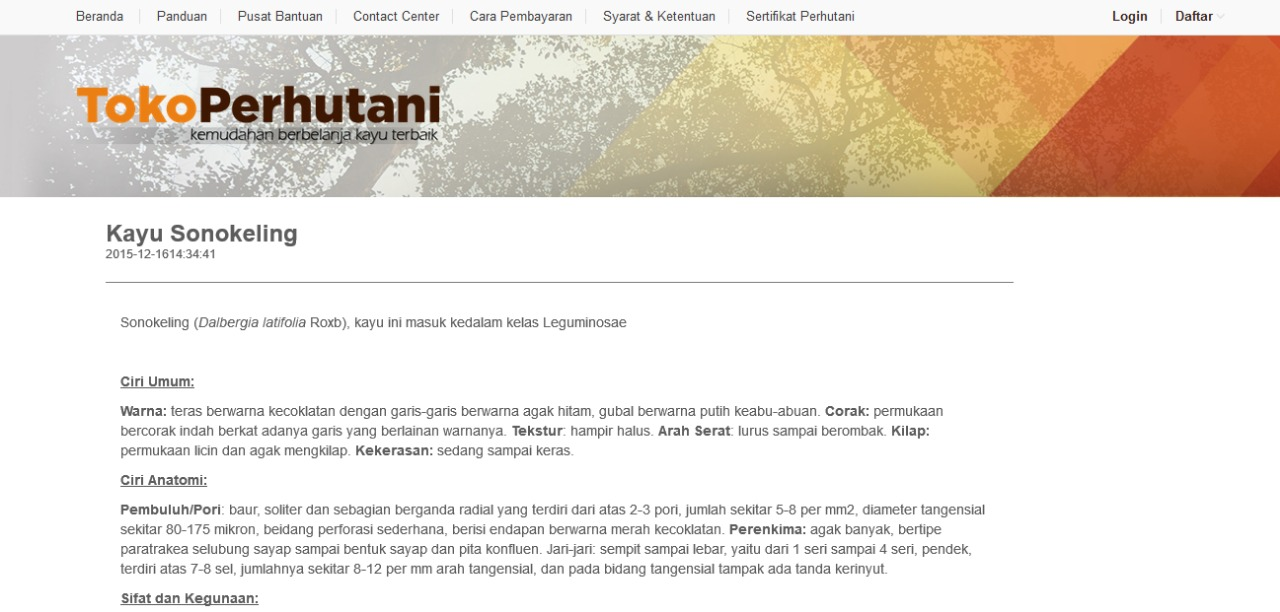
\includegraphics[scale=0.3]{figures/j3}
\caption{Kayu Sonokeling}
\end{figure}